\documentclass[12pt,english]{scrartcl}

\usepackage{amsmath,amssymb}
\usepackage[amssymb]{SIunits}
\usepackage{babel}
\usepackage[latin1]{inputenc}
\usepackage{graphicx}

\title{KOGW-PM-KNP: Edge detection I - Gaussian filtering}
\author{}
\date{\today}

\begin{document}
%Hier kommt der Dokumententext

\maketitle

Complete the tasks using python. Your answers should include the code you wrote and written answers to the questions with relevant output images.

\section*{Task 1. Gaussian filtering of an image}

\begin{figure*}[htbp]
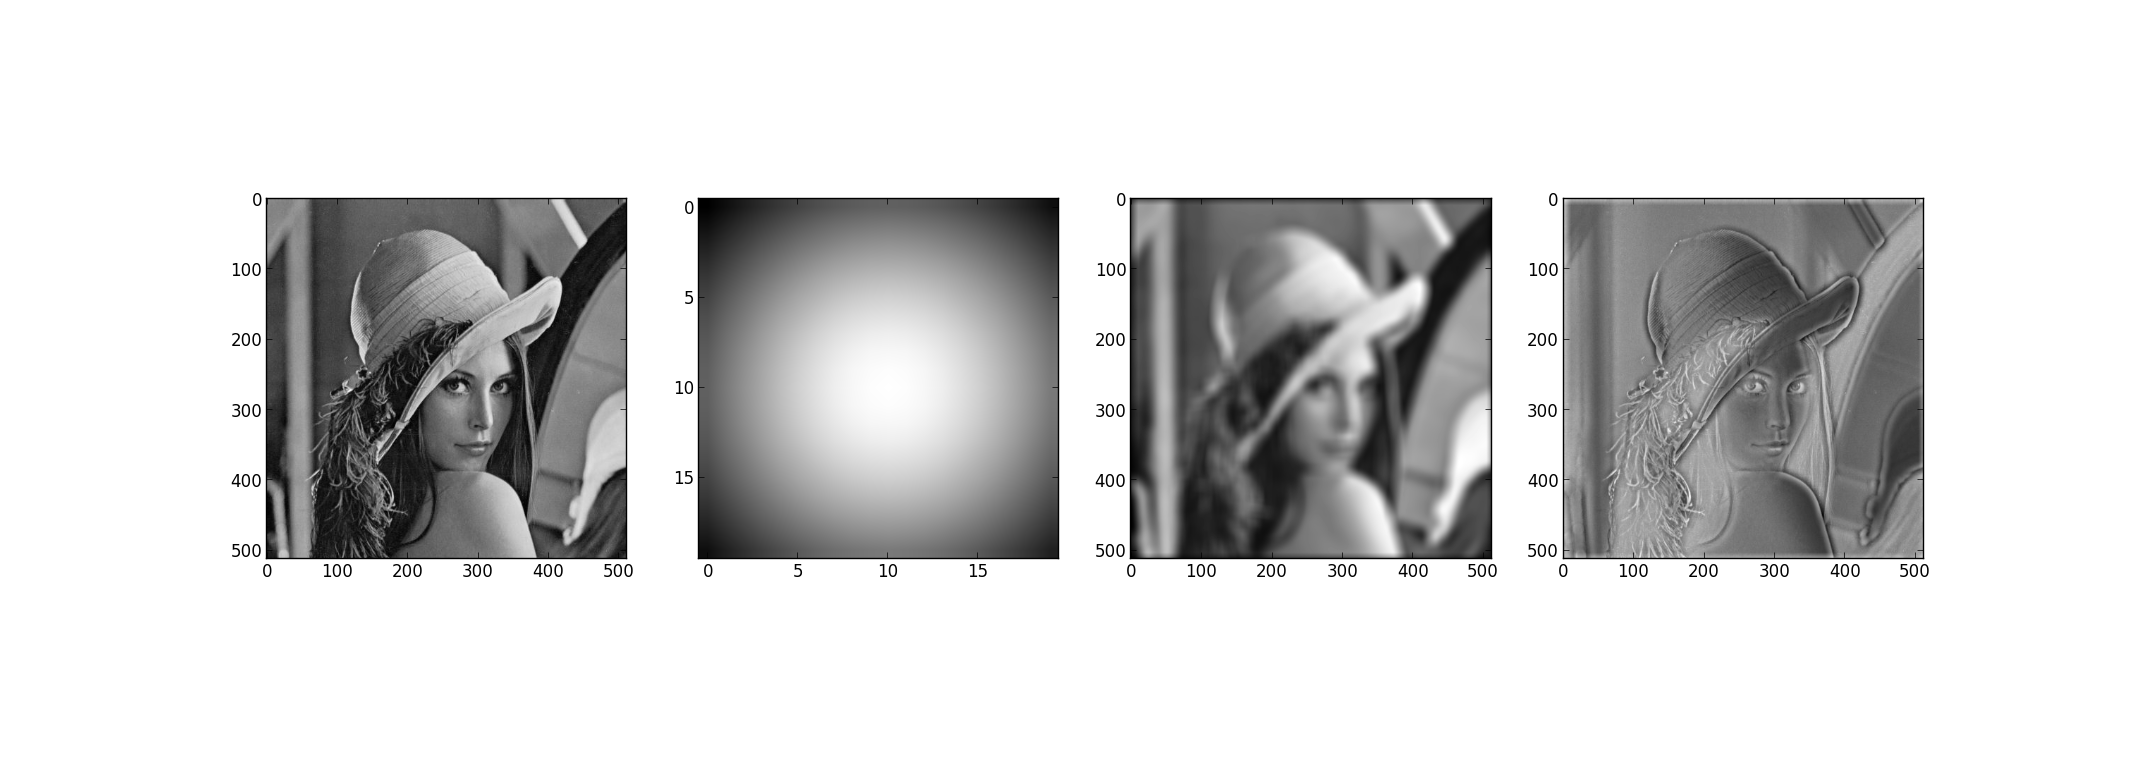
\includegraphics[width=1.0\textwidth]{Figures/Edge_detection_1/Figure1ED.png}
\caption{From left to right: original image, Gaussian filter, blurred image resulting from convolution of original image with Gaussian filter,   output/ edge-detected output}
\label{fig:lena_gauss}
\end{figure*}

\begin{enumerate}
 \item Using the given equation for a 2D Gaussian filter, plot the output of a filter-convolved image with an appropriate sigma $\sigma$ value.
 \item[] $G(x,y) = \frac{1}{2\pi\sigma^2} *e^{-\frac{x^2+y^2}{2\sigma^2}}$
 \item What type of filter results from a high $\sigma$ value? 
 \item Can you think of a way of extracting high frequency components from an image using only a low frequency filtered image? Plot such an image and comment on its quality
 \item[]
 \item[] \textit{Hint: Use PIL.Image.open to import your image, and from scipy.signal use the convolve2d (with mode='same') function for the convolution.}
\end{enumerate}

 

\section*{Task 2. Difference of Gaussian filtering of an image}

\begin{enumerate}
 \item Create a Difference of Gaussian (DOG) filter by applying two different sigma valued Gaussian filters to the original image and then subtracting the two outputs from each other.
 \item Try to find optimum sigma values for detecting edges in an image.
 \item Comment on differences between this filter and the first.
\end{enumerate}
\begin{figure*}[htbp]
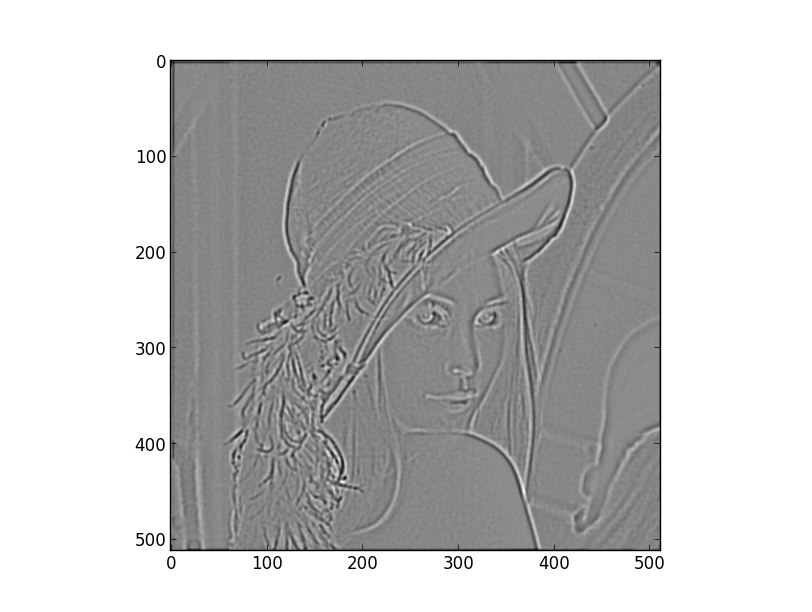
\includegraphics[width=0.3\textwidth]{Figures/Edge_detection_1/Figure2ED.png}
\caption{Add text to describe the different panels}
\label{fig:lena_edge}
\end{figure*}

 
\end{document}